\documentclass[11pt]{article}
\usepackage[utf8]{inputenc}
\usepackage{amsmath,amssymb,hyperref,array,xcolor,multicol,verbatim,mathpazo}
\usepackage[normalem]{ulem}
\usepackage[pdftex]{graphicx}
\setlength{\parskip}{2\baselineskip}
\usepackage[margin=1in]{geometry}
\usepackage{pdfpages}

\usepackage[style=apa]{biblatex}
\addbibresource{./report.bib}

\usepackage{graphicx}
\graphicspath{ {./report_images/} }

\input tikz.tex
\usetikzlibrary{cd}
\usepackage{adjustbox}

\begin{document}

\title{Choices of Invariants for SE(3) Equivariant Attention Mechanisms}
\author{Niklas Mather}
\maketitle

\section{Introduction}

Attention mechanisms are a neural network layer which parameterise the interactions between different inputs to a neural network by the features associated with those inputs. One of their benefits is that they make very few assumptions about the global domain structure, and so provide a recipe that generalises easily to new domains. As such, it has been successfully applied on problems raning from natural language processing (\cite{vaswani2017attention}) to protein-protein interactions (\cite{velivckovic2017graph}) and machine vision tasks (\cite{vision_transformer}). While this generality is useful, it is at odds with a competing objective of neural network design: to leverage prior knowledge of the domain structure for better performance .

For example, group-equivariant neural networks use knowledge of the symmetries of the input domain to reduce generalisation error (\cite{volumetric}) and reduce sample complexity (\cite{winkels2019pulmonary}). This approach relies on constraining the forms of the layers in a given neural network so that they are 'equivariant' with respect to symmetry transformations, and has been extended to include equivariant attention mechanisms, which achieve competitive performance with standard convolutional group-equivariant networks on a number of benchmarks.
  
These group-equivariant attention mechanisms are the focus of this paper. Specifically, we build on previous work that solved for the equivariance constraints in the case of the standard Euclidean group in 3 dimensions (SE(3)) (\cite*{volumetric} and \cite*{rototranslational}). Within this framework, there are still a number of design choices available to the user, especially in how to paramaterise the group invariants. The focus of our paper will be on the impact of these design choices.

The work is divided into three sections: \begin{itemize}
	\item A summary of the theory of group-equivariant attention mechanisms and a precise statement of the problem.
	\item A demonstration of how equivariance arises from integral transforms, from the perspective of category theory.
	\item An ablation study of the impact of different choices of group invariants on the MD17 dataset. 
\end{itemize}

\section{Mathematical Background}
\subsection*{Functions on point clouds of homogeneous spaces}

We are concerned with constructing neural networks that can leverage data that exists as a point cloud on a homogeneous space $X$, corresponding to some group $G_X$. A homogeneous space is defined as the set of points on which its corresponding group acts transitively. That is: 

$$ X = \{x \in X | x = g \cdot y, y \in X, g \in G_X \} $$

The notation $g \cdot x$ denotes a group element 'acting' on $x$. Formally, such a group action is a bijective function, from $X$ to itself, also known as an automorphism of $X$. We also denote:

$$ \text{Aut}(X) = \{T: X \rightarrow X | X \text{ is a bijection } \}$$

Where by definition we require that the map $T: G \rightarrow \text{Aut}(X)$ is an injective group homomorphism, that is $T(gh)=T(g)T(h) \forall g, h \in G_X$. Because not all groups are abelian, we must technically distinguish between 'left' and 'right' actions, which differ in whether $h$ or $g$ acts on $x$ first during the action of the product $gh$. However, in this paper I will always refer to left actions, where $T_{gh} (x) = T_g (T_h (x))$.

A \textbf{point cloud} is a discrete subset of $X$, which I will denote $\tilde{X}$. It is common to also consider the points as the vertices of a graph that is embedded in $X$. That is, given a point $x \in  \tilde{X}$, there is a set $N(x) \subset \tilde{X}$ of points which share an edge with $x$ - called the neighbourhood of $x$ - which share an edge with $x$. This graph may or may not have any true semantic meaning, but in either case gives us a convenient notation with which to describe pairwise relationships between specific points.

Throughout this paper, I will reference molecular chemistry as a running example of the type of problem I am trying to solve. A molecule is a set of points (atoms) which are distributed through three-dimensional space. That is, one molecule's position differs from another by the action of a translation on their coordinate vectors. Moreover, while atoms may be rotationally symmetric, \textit{pairs} of atoms may differ by a 3d rotation. Thus, a molecule is a discrete set of points distributed on a manifold corresponding the group generated by all 3d rotations and translations, also known as SE(3).   

\subsection{Feature fields}
Of course, molecules are defined by other types of properties than their raw location. For example, each atom belongs to an elemental class which defines how it interacts with other atoms. Moreover, each atom may have geometric quantities with it (e.g. the sum of all force vectors acting on it). We refer to these as \textbf{features} defined on the point cloud.

%TODO talk about why this is useful.
These features could be described as a vector-valued function on a point cloud, but it is more natural and useful to define them as functions over the underlying space if we expect them to be continuous on that domain. The two perspectives can be made compatible in the following way: given a function $f: X \mapsto Y$ we can define a function $f': \tilde{X} \mapsto Y$ which by construction has $f'(x) = f(x) \forall x \in \tilde{X}$.

$$ f'(x) := \sum_j f(x_j)\delta_(x - x_j)$$

\section{Equivariance from a categorical perspective}

\subsection*{Features, Functions and Integral Transforms}

Given a manifold $X$ and $Y$, we can define an associated space of functions:

$$ F(X) := \{ f: X \rightarrow \mathbb{R}^d \}$$

As stated above, we are interested in constructing equivariant maps between such spaces. Three natural questions are:

\begin{itemize}
    \item How do we ensure that a given transform is equivariant?
    \item How do we ensure that an attention layer is equivariant?
    \item Can we generalise this construction beyond the case where Aut$(X)$ are group actions?
\end{itemize}

The first of these two have been answered in the literature before, but I took a slightly different route to establishing them, using a construction of integral transforms from category theory. I will now describe this construction here and show how it can be used to answer the questions above. This section was heavily influenced by the discussion in \cite{integral_transforms}

We are given two spaces: $X$ and $Y$. For each of these we may define a space of functions $F(X)$ and $F(Y)$, and our goal is to construct a map $K: F(X) -> F(Y)$

First, consider the product space and the associated projection maps:

$$ p(x, y) = x, \ \  q(x, y) = y$$

\pagebreak

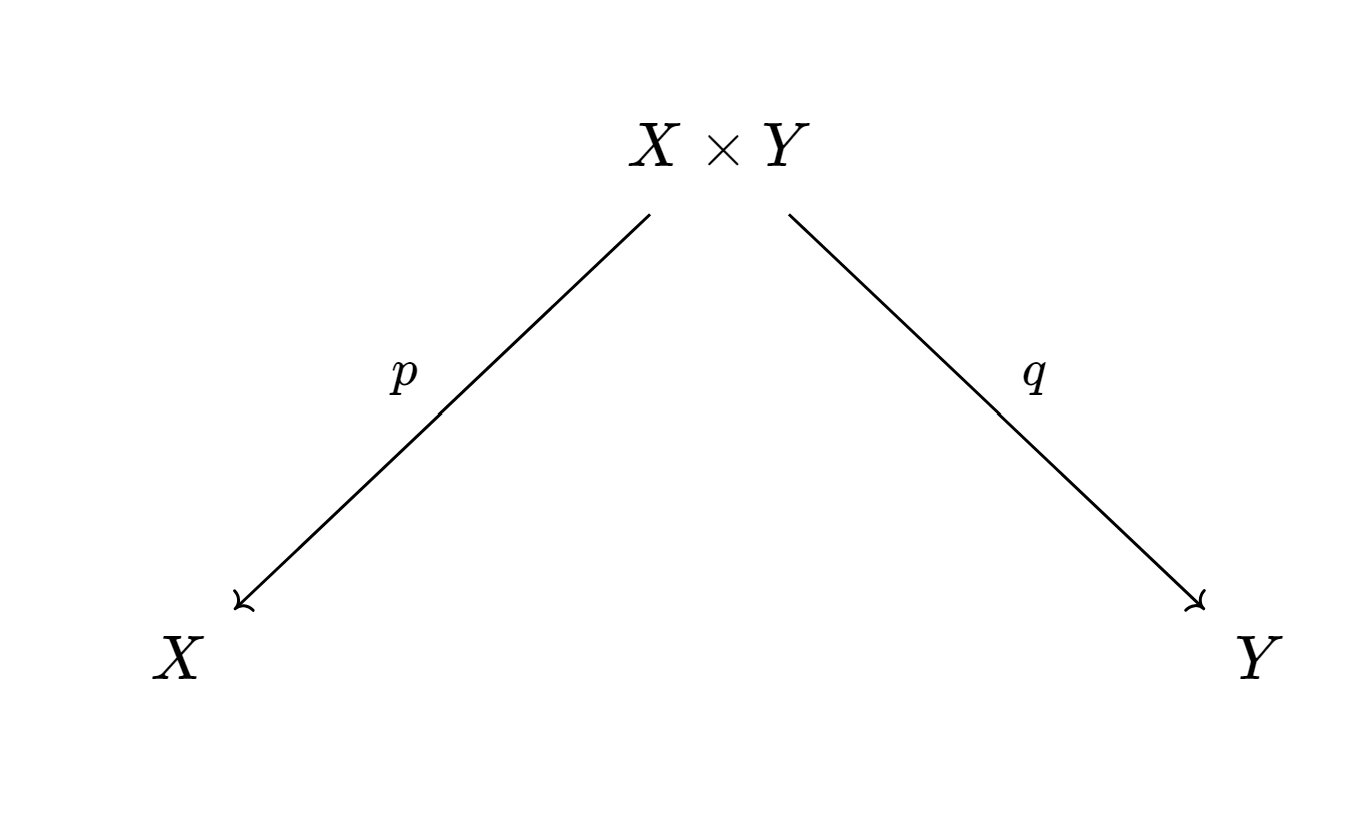
\includegraphics[scale=0.4]{basic_span.png}

Now, we can use $p$ to construct a map from $F(X)$ to $F(X\times Y)$ via precomposition. That is, given a function $f \in F(X)$, there is a unique function $\tilde{f}(x,y) = f \circ p (x, y)  \in F(X \times Y)$. Denoting precomposition as $p^*$ we have obtained a map $p^*: F(X) \rightarrow F(X) \times Y$. In category theory, this map is referred to as the 'pull-back'.

How can we construct a map from $F(X \times Y)$ to $F(Y)$? Our goal is to 'remove' the dependence on $x$ for a given function $f(x, y)$. Thus we must aggregate over the fibres of the projection map $q^{-1}(y)$. There are many possible aggregation functions, but in keeping with the standard definiton of the integral transform I will here use integration. Thus we have defined the 'push-forward' $q_* : F(X \times Y)$.

$$ (q_* f)(y) = \int_{q^{-1}(y)} f(x, y) dx $$

Finally, we note that multiplication by a kernel is a transformation 
$$k \cdot : F(X) \times Y \rightarrow F(X \times Y)$$ 

Thus, we have the following diagram:

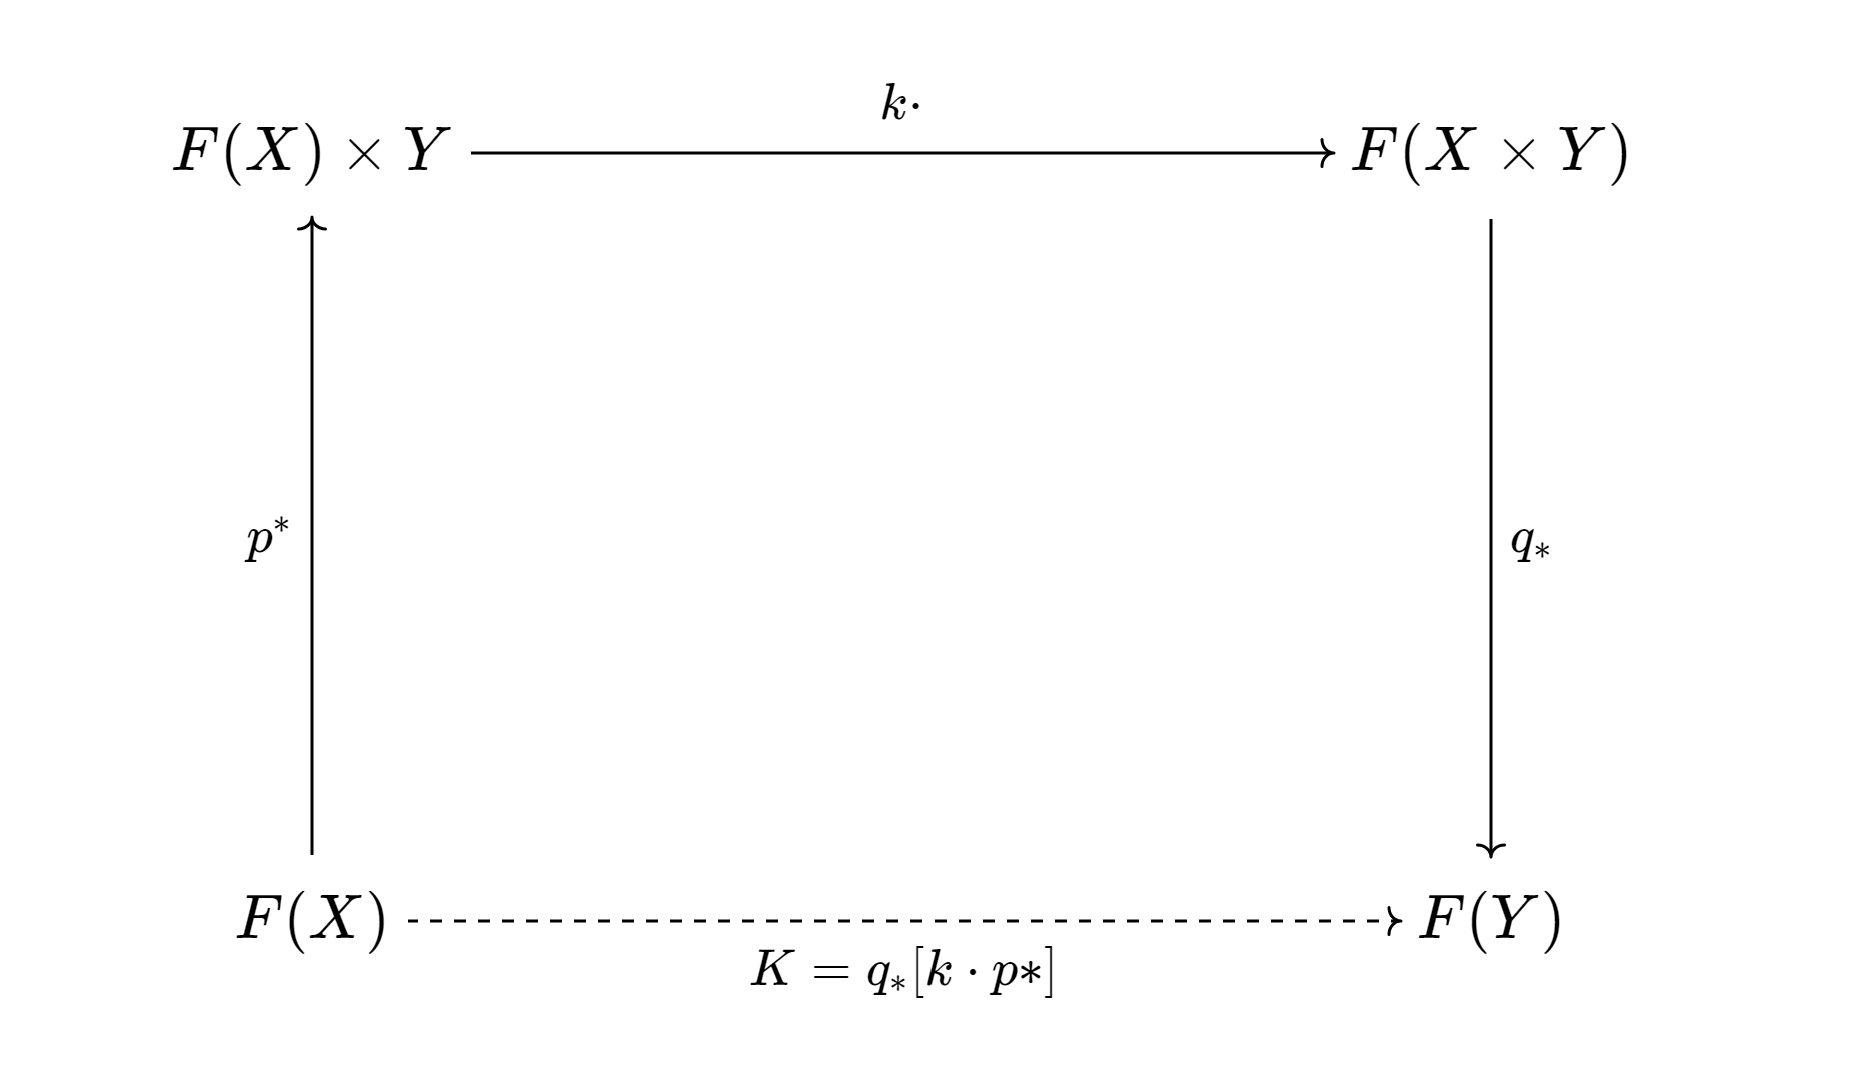
\includegraphics[scale=0.4]{integral_transform_diagram.png}

\subsubsection*{Constructing Equivariant Integral Transforms}

The above diagram characterises all possible linear transformations from $F(X)$ to $F(Y)$, but we are explicitly considered in those that that commute with morphisms of the category $F(X)$. If $X$ is a homogeneous space and the morphisms are group actions, this corresponds to solving for the equivariance constraints.

Suppose we have two transformations $T_X: X \mapsto Y$ and $T_Y: Y \mapsto Y$. Each of these lift to actions $\tilde{T}_X: F(X) \mapsto F(X)$ and $\tilde{T}_Y: F(Y) \mapsto F(Y)$, given by $\tilde{T}_X f(x) := f(T(x))$. Under what circumstances does $K T_X f = T_Y K f$ for every choice of $f$?

Choose any $f \in F(X)$. Then, the commutativity condition gives:

\begin{align*}
  K \tilde{T}_X f &= \tilde{T}_Y K f \\
  q_* k \cdot p^*\tilde{T}_X f (y) f &= q_* k \cdot p^* f (T_Y(y)) \\
  \int_{q^{-1}(y)} k(x, y) f(T_X(x)) dx &= \int_{q^{-1}(T_Y(y))} k(x, T_Y(y)) f(x) dx \\
  \int_{q^{-1}(y)} k(T_X^{-1}(x), y) f(x) dx &= \int_{q^{-1}(T_Y(y))} k(x, T_Y(y)) f(x) dx 
\end{align*}


Now, under the condition that the fibres (considered as sets) are invariant under the group action:

$$ q^{-1}(y) = q^{-1}(T_Y(y)) $$

We can equate the terms under the integral signs using the fundamental theorem of calculus:

$$ k(T^{-1}_X(x), y) f(x) = k(x, T_Y(y)) f(x)  $$

Choosing in particular the case where $f$ is a constant function, we have:

\begin{align*}
	k(T^{-1}_X(x), y) &= k(x, T_Y(y)) \\
	k(x, y) &= k(T_X(x), T_Y(y))
\end{align*}

Therefore, we see that there is a correspondence between $\tilde{T}_X$ and $\tilde{T}_Y$ as long as $k$ is constant on the curves in the product space $X \times Y$ induced by $T_X$ and $T_Y$. In the case when $X$ and $Y$ are homogeneous spaces corresponding to the same group, and $T_X = T_Y$, this recovers the standard result that a group action commutes with an integral transform if $k(x, y) = k(0, I(x,y))$ for some function $I$ that is invariant under the group action. 

\subsection*{Visual Intuition}

This construction also affords us some interesting visual intuition of how equivariance is achieved. Consider the following illustration of $F(X) \times Y$ and $F(X \times Y)$.

\subsection*{Attention Mechanisms as Integral Transforms}

Our original goal was to understand how attention mechanisms could be made equivariant. This can be acheived straightforwardly using the compositional construction. We only have to modify the definition of $q$ so that it maps from the set of neighbours of a vertex to the vertex itself:

$$ q^{-1}(y) := N(y)$$

Then, the fibres $q^{-1}(y)$ are once again invariant under the group structure, and we can repeat the argument above.

Moreover, the coefficients $\alpha_{ij}$ define a kernel $k(x_i, y_j)$. As long as these coefficients are invariant under group actions, the attention layer will be equivariant. Under what conditions will this be true?

%TODO MORE - NEED TO DESCRIBE THE RELATIONSHIP BETWEEN EQUIVARIANCE IN K AND Q AND INVARIANCE IN ALPHA

\subsection*{Discussion: does this generalise beyond groups?}

% TODO MORE

In the above discussion, I deliberately avoided referencing the transformations as group actions. It's worth pausing to consider whether groups are the only categories for which we could construct layers that commute with the morphisms of that category. 


\section{Ablation Study on SE(3)}

In this section, I describe an ablation study that was run on SE(3) and the MD17 dataset. The goal was to see whether different paramaterisations of the group invariants in the attention mechanism could be used as an inductive bias. In constructing my model, I broadly followed the recipe laid out by (REF: roto translational), but re-implemented the model from scratch in the PyTorch Geometric framework (REF: PyG). All code can be found in: \href{https://github.com/nsmat/transformer_invariants}.

\subsection*{Equivariant maps in the SE(3) context}

The standard Euclidean group in 3 dimensions comprises all rotations and reflections of $\mathbb{R}^3$. This group is the natural way to define weight sharing when studying molecular systems, because molecules have the same properties regardless of their position or orientation in space.

To construct an SE(3) equivariant attention mechanism, we need to decide how we will represent both node features (which represent information about a single atom) and edge level features (which represent information about pairs of atoms). In our notation features. We are ultimately interested in modelling directional forces acting on each atom, and so a natural choice is to represent the node features as functions defined over the possible orientations in $\mathbb{R}^3$  - or equivalently over the sphere $S^2$. Such functions can be represented as a linear combination of spherical harmonics, which have two desirable properties: first, that they form an orthonormal basis (with respect to the standard L2 inner product) for functions on $S^2$, and second that they transform equivariantly under rotations.

The edge features similarly should carry geometric information. However, they are distinct from node features in that they should vary as we change the distance between the two nodes. In our model, this is acheived by computing the edge features using a tensor product between the node features of the neighbour, and the Fourier representation of the relative position of two nodes. The weights of the tensor product are obtained via an MLP that takes the distance between the two nodes as input.

To summarise, each component of our attention mechanism is computed in the following manner:

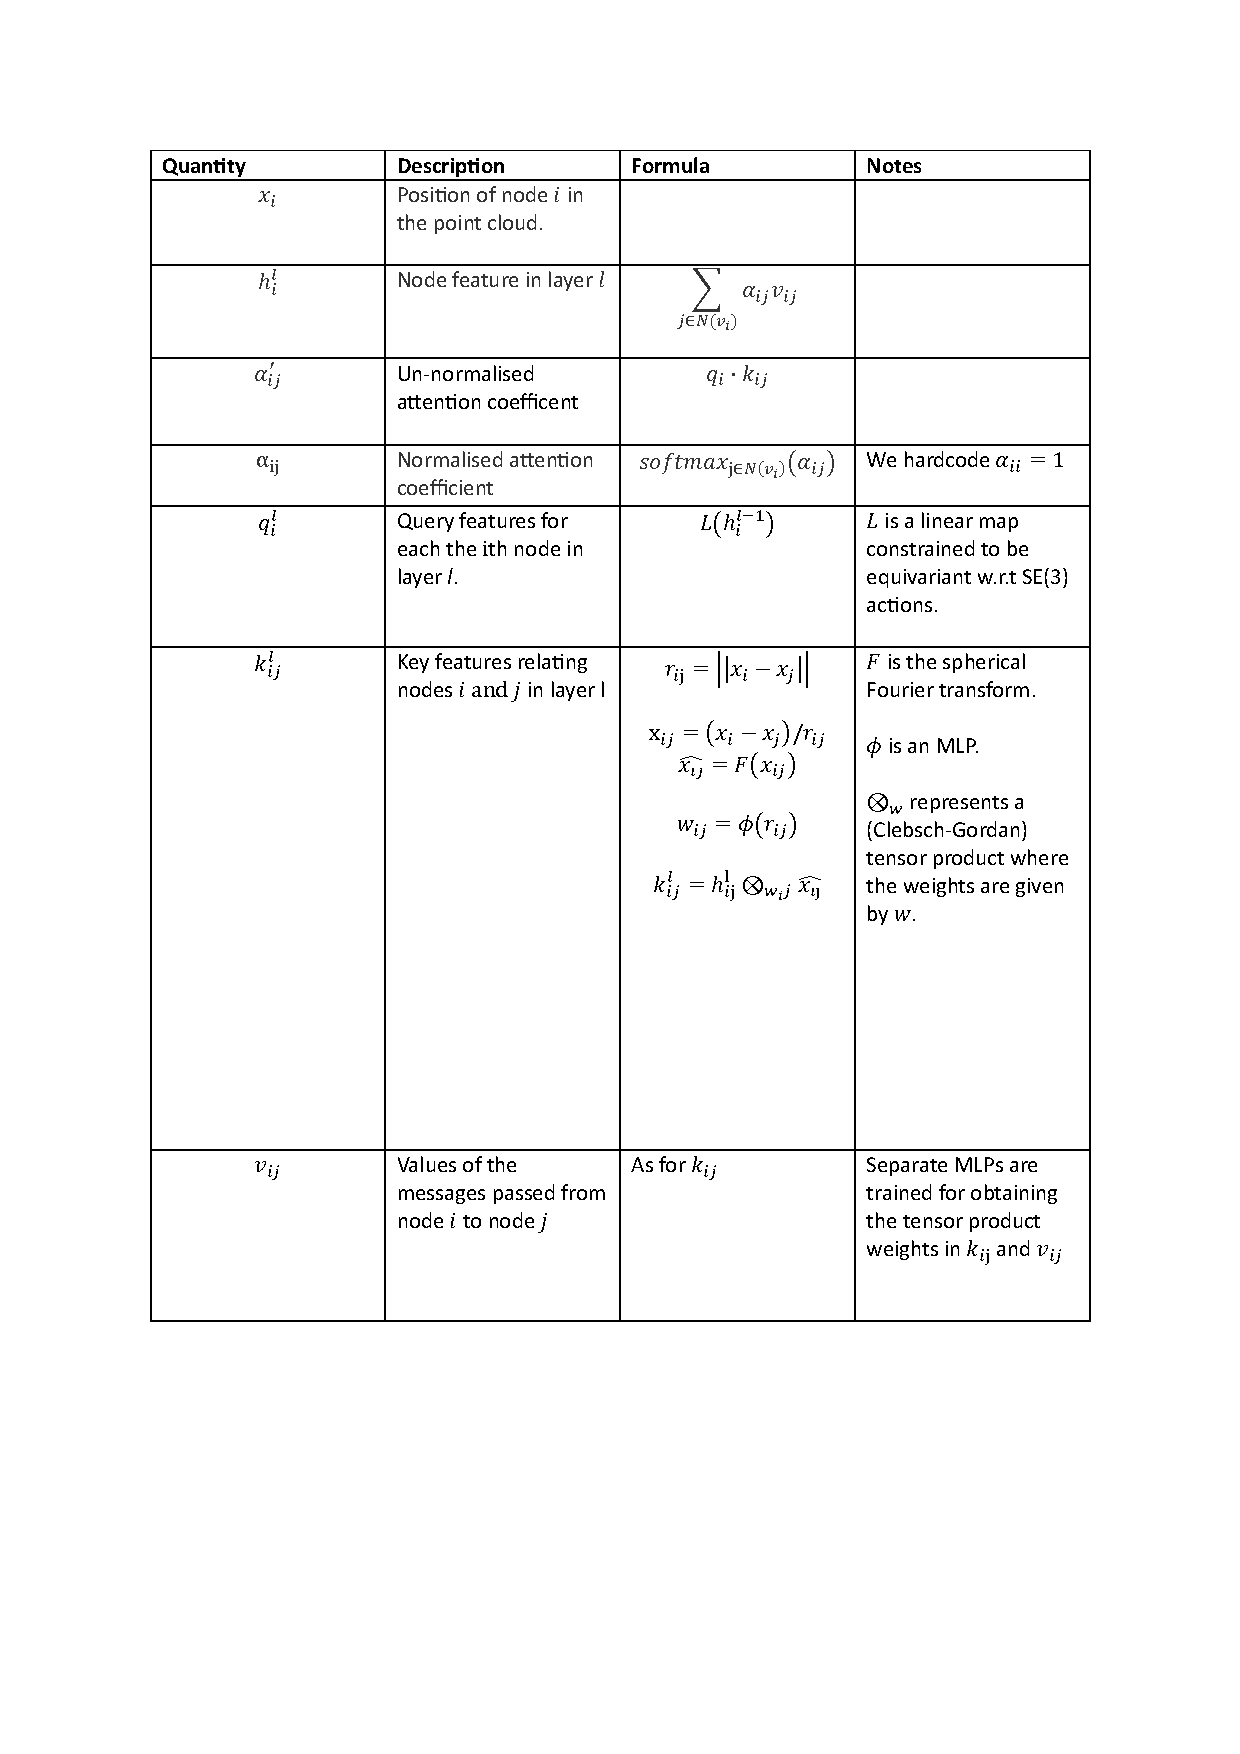
\includepdf{report_images/quantity_table.pdf}

\subsection{Architecture design}

In each of the following experiments, we used a multi-headed, multi-layer transformer architecure. Derived equivariant features were calculated separately in each head, then concatenated to form the final latent representation of the graph. Finally, the equivariant features were mapped to a set of type-0 features, creating a transformation invariant representation of the molecule.

We used 4 attention heads, each with 4 layers. Each layer used 8 channels of type-0, type-1 and type-3 features, following the recommendation given in (\cite{rototranslational}). Internally, the tensor-product weight functions are paramaterised as multi-layer perceptrons with 32 hidden units. These are the only source of non-linearity in the network, and since distances are naturally SE(3) invariant, all layers remain equivariant when using standard activation functions.

Rather than use a fully-connected graph, which is typical of transformer architecures, the input graphs were derived during pre-processing by connecting nodes that were within 2 angstroms of each other. This reduces inference time in each pass of the neural network, allowing for a larger number of epochs during training.  

All tensor products and equivariant linear maps were implemented using the e3nn library (\cite{geiger2022e3nn}).

All models were trained for 12 hours on an Nvidia A100 GPU using a batch size of 64.

\subsection{Results}

We tested three choices of paramaterisation of the distance: the standard Euclidean norm, the inverse of the standard Euclidean norm, and a 'mixed-model' where half the heads use the first of these and half the heads use the second.

\section{Conclusion}

\end{document}